\documentclass[a4paper,12pt]{article}



%%% Работа с русским языком
			% кодировка
\usepackage[utf8]{inputenc} 
\usepackage[T2A]{fontenc}	
\usepackage[english,russian]{babel}   %% загружает пакет многоязыковой вёрстки
%\usepackage{pscyr} % Нормальные шрифты
\usepackage{cmap}
\usepackage{algorithm}
\usepackage{algorithmic} 
\usepackage{indentfirst}
\usepackage{xcolor}
\usepackage{hyperref}

 % Цвета для гиперссылок
\definecolor{linkcolor}{HTML}{799B03} % цвет ссылок
\definecolor{urlcolor}{HTML}{799B03} % цвет гиперссылок

\hypersetup{pdfstartview=FitH,  linkcolor=linkcolor,urlcolor=urlcolor, colorlinks=true}
%%% Дополнительная работа с математикой
\usepackage{amsmath,amsfonts,amssymb,amsthm,mathtools} % AMS
\usepackage{amsfonts}
\usepackage[miktex]{gnuplottex} % <- Use instead if running TeX Live.

\usepackage{icomma} % "Умная" запятая: $0,2$ --- число, $0, 2$ --- перечисление
%% Номера формул
%\mathtoolsset{showonlyrefs=true} % Показывать номера только у тех формул, на которые есть \eqref{} в тексте.
%\usepackage{leqno} % Нумерация формул слева

%% Свои команды
\DeclareMathOperator{\sgn}{\mathop{sgn}}

%% Перенос знаков в формулах (по Львовскому)
\newcommand*{\hm}[1]{#1\nobreak\discretionary{}
	{\hbox{$\mathsurround=0pt #1$}}{}}

%%% Работа с картинками
\usepackage{graphicx}  % Для вставки рисунков
\usepackage{calc}
\usepackage{subcaption}
\graphicspath{{images/}{images2/}}  % папки с картинками
\setlength\fboxsep{3pt} % Отступ рамки \fbox{} от рисунка
\setlength\fboxrule{1pt} % Толщина линий рамки \fbox{}
\usepackage{wrapfig} % Обтекание рисунков текстом

%%% Работа с таблицами
\usepackage{array,tabularx,tabulary,booktabs} % Дополнительная работа с таблицами
\usepackage{longtable}  % Длинные таблицы
\usepackage{multirow} % Слияние строк в таблице

%%% Теоремы
\theoremstyle{plain} % Это стиль по умолчанию, его можно не переопределять.
\newtheorem{theorem}{Теорема}[section]
\newtheorem{proposition}[theorem]{Утверждение}
\newtheorem{problem}{Задача}[section]

\theoremstyle{definition} % "Определение"
\newtheorem{lemma}{Лемма}[section]
\newtheorem{conclusion}{Следствие}[theorem]

\theoremstyle{remark} % "Примечание"
\newtheorem*{nonum}{Определение}

%%% Программирование
\usepackage{etoolbox} % логические операторы

%%% Страница
\usepackage{geometry} % Простой способ задавать поля
\geometry{top=30mm}
\geometry{bottom=40mm}
\geometry{left=20mm}
\geometry{right=20mm}

%\usepackage{fancyhdr} % Колонтитулы
% 	\pagestyle{fancy}
%\renewcommand{\headrulewidth}{0pt}  % Толщина линейки, отчеркивающей верхний колонтитул
% 	\lfoot{Нижний левый}
% 	\rfoot{Нижний правый}
% 	\rhead{Верхний правый}
% 	\chead{Верхний в центре}
% 	\lhead{Верхний левый}
%	\cfoot{Нижний в центре} % По умолчанию здесь номер страницы
\usepackage[normalem]{ulem}  % для зачекивания текста
\usepackage{setspace} % Интерлиньяж
\onehalfspacing % Интерлиньяж 1.5
%\doublespacing % Интерлиньяж 2

\usepackage{tikz}
\usetikzlibrary{arrows}
\usepackage{lastpage} % Узнать, сколько всего страниц в документе.
\usepackage{soul} % Модификаторы начертания

\usepackage{color}
\usepackage{colortbl}
\usepackage{upgreek}
\usepackage{hyperref}
\usepackage{amsmath,amsfonts,amsthm,amssymb,amsbsy,amstext,amscd,amsxtra,multicol}
\usepackage{indentfirst}
\usepackage{verbatim}
\usepackage{tikz} %Рисование автоматов
\usetikzlibrary{automata,positioning}
\usepackage{multicol} %Несколько колонок
\usepackage{graphicx}
%% \voffset-5mm
%% \def\baselinestretch{1.44}
\renewcommand{\theequation}{\arabic{equation}}
\def\hm#1{#1\nobreak\discretionary{}{\hbox{$#1$}}{}}
\newtheorem{Lemma}{Лемма}
\newtheorem{Remark}{Замечание}
%%\newtheorem{Def}{Определение}
\newtheorem{Claim}{Утверждение}
\newtheorem{Cor}{Следствие}
\newtheorem{Theorem}{Теорема}
\theoremstyle{definition}
\newtheorem{Example}{Пример}
\newtheorem*{known}{Теорема}
\def\proofname{Доказательство}
\theoremstyle{definition}
\newtheorem{Def}{Определение}

%% \newenvironment{Example} % имя окружения
%% {\par\noindent{\bf Пример.}} % команды для \begin
%% {\hfill$\scriptstyle\qed$} % команды для \end


%\date{22 июня 2011 г.}
\let\leq\leqslant
\let\geq\geqslant
\def\MT{\mathrm{MT}}
%Обозначения ``ажуром''
\def\BB{\mathbb B}
\def\CC{\mathbb C}
\def\RR{\mathbb R}
\def\SS{\mathbb S}
\def\ZZ{\mathbb Z}
\def\NN{\mathbb N}
\def\FF{\mathbb F}
%греческие буквы
\let\epsilon\varepsilon
\let\es\emptyset
\let\eps\varepsilon
\let\al\alpha
\let\sg\sigma
\let\ga\gamma
\let\ph\varphi
\let\om\omega
\let\ld\lambda
\let\Ld\Lambda
\let\vk\varkappa
\let\Om\Omega
\def\abstractname{}

\def\R{{\cal R}}
\def\A{{\cal A}}
\def\B{{\cal B}}
\def\C{{\cal C}}
\def\D{{\cal D}}
\let\w\omega

%классы сложности
\def\REG{{\mathsf{REG}}}
\def\CFL{{\mathsf{CFL}}}
\newcounter{uproblem}
\newcounter{subproblem}
\def\pr{\medskip\noindent\stepcounter{problem}{\bf \theproblem .  }\setcounter{subproblem}{0} }
\def\prp{\medskip\noindent\stepcounter{problem}{\bf Задача \theproblem .  }\setcounter{subproblem}{0} }
\def\prstar{\medskip\noindent\stepcounter{problem}{\bf Задача $\theproblem^*$ .  }\setcounter{subproblem}{0} }
\def\prdag{\medskip\noindent\stepcounter{problem}{\bf Задача $\theproblem^\dagger$ .  }\setcounter{subproblem}{0} }
\def\upr{\medskip\noindent\stepcounter{uproblem}{\bf Упражнение \theuproblem .  }\setcounter{subproblem}{0} }
%\def\prp{\vspace{5pt}\stepcounter{problem}{\bf Задача \theproblem .  } }
%\def\prs{\vspace{5pt}\stepcounter{problem}{\bf \theproblem .*   }
\def\prsub{\medskip\noindent\stepcounter{subproblem}{\rm \thesubproblem .  } }
%прочее
\def\quotient{\backslash\negthickspace\sim}
\usepackage{csquotes} % Еще инструменты для ссылок
\usepackage{listings}

\newcolumntype{g}{>{\columncolor{Gray}}c}
\newcolumntype{d}{>{\columncolor{darkishgreen}}c}

\author{Сотников А.Д, Северилов П.А.}
\title{Решение уравнения Пуассона методом быстрого преобразования Фурье}
\date{}
\begin{document}
\maketitle

\begin{abstract}
	В проекте описывается реализация решения двумерного уравнения Пуассона методом быстрого преобразования Фурье на языке программирования Python 3.

\end{abstract}

\textbf{Ключевые слова}: \emph {уравнение Пуассона, быстрое преобразование Фурье (FFT), уравнения в частных производных, граничные условия}.

	\section{Преобразование Фурье}
	\subsection{DTF}
		Вспомним, что мы хотим вычислить полином
		$$A(x)=\sum_{j=0}^{n-1}a_{j}x^{j}$$
		с границей степени $n$ в точках $\omega_{n}^{0}, \omega_{n}^{1}, \omega_{n}^{2}, \dots, \omega_{n}^{n-1}$, которые представляют собой $n$ комплексных корней $n$--степени из единицы. Пусть полином $A$ задан в форме коэффициентов: $a=(a_{0}, a_{1},\dots, a_{n-1})$. Определим результат $y_{k}$, где $k=0,1,\dots,n-1$, с помощью формулы
		$$y_{k}=A(\omega_{n}^{k})=\sum_{j=0}^{n-1}a_{j}\omega_{n}^{kj}.$$
		Вектор $y=(y_{0}, y_{1}, \dots, y_{n-1})$ представляет собой \textrm{\textbf{\textit{дискретное преобразование Фурье.}}}
		\medskip
		
	\subsection{FFT}
		С помощью \textrm{\textbf{\textit{быстрого преобразования Фурье (FFT)}}}, вычисления можно проводить за $\Theta(n\lg n)$, где $n$ -- точная степень 2. В методе FFT применяется стратегия декомпозиции, в которой отдельно используются коэффициенты полинома $A(x)$ с четными и нечетными индексами:
		$$A^{[0]}(x)=a_{0}+a_{2}x+a_{4}x^{2}+\cdots+a_{n-2}x^{n/2-1},$$
		
		$$A^{[1]}(x)=a_{1}+a_{3}x+a_{5}x^{2}+\cdots+a_{n-1}x^{n/2-1}.$$
		
		Такая декомпозиция является основой следующего рекурсивного алгоритма FFT:

		\begin{algorithm}[h!]
			\caption{Recursive-FFT(a)}
			\label{Rec-FFT}
			\begin{algorithmic}[1]
				\STATE n = a.length \ \ \ \ \ // \text{$n$ является степенью 2}
				\IF {$n==1$}
				\RETURN $a$
				\ENDIF
				\STATE $\omega_{n}=e^{2\pi i/n}$
				\STATE $\omega=1$
				\STATE $a^{[0]}=((a_{0}, a_{2},\dots, a_{n-2}))$
				\STATE $a^{[1]}=((a_{1}, a_{3},\dots, a_{n-1}))$
				\STATE $y^{[0]}= \ $Recursive-FFT($a^{[0]}$)
				\STATE $y^{[1]}= \ $Recursive-FFT($a^{[1]}$)
				\FOR {$k=0 \  \textbf{to} \ n/2-1$}
				\STATE $y_{k}=y_{k}^{[0]}+\omega y_{k}^{[1]}$
				\STATE $y_{k+(n/2)}=y_{k}^{[0]}-\omega y_{k}^{[1]}$
				\STATE $\omega$ = $\omega\omega_{n}$
				\ENDFOR
				\RETURN y \ \ \ \ \ // \text{Считаем, что $y$--вектор-столбец}
				
			\end{algorithmic}
		\end{algorithm}
	
	Видно, что в строчках 11-15 алгоритм дважды вычисляет выражение $\omega_{n}^{k}y_{k}^{[1]}.$ Можно изменить цикл так, чтобы вычислять это значение только один раз, сохраняя его во временной переменной $t$. Такой прием называется \textrm{\textbf{\textit{преобразованием бабочки}}}. Иллюстрацию работы алгоритма можно посмотреть на рис.1.
	
	
	
	\begin{figure}[H]
		\center{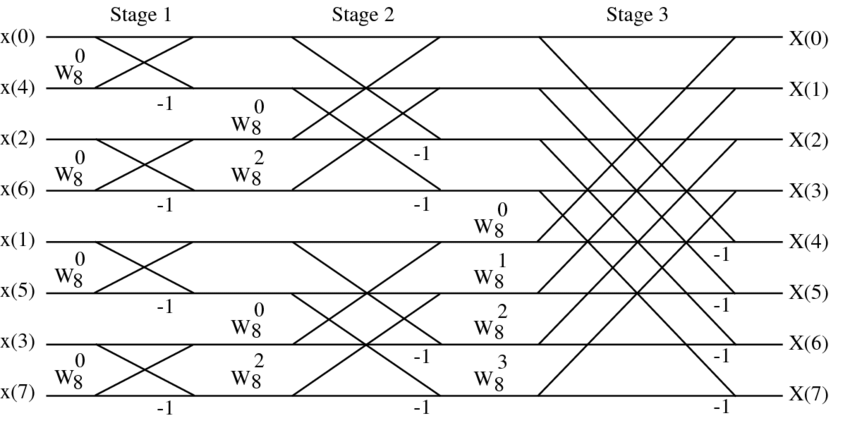
\includegraphics[width=0.8\linewidth]{theory/fft-butterfly.png}}
		\caption{Схема FFT с преобразованием бабочки.}
	\end{figure}

	С использованием данной операции рекурсивный метод можно ускорить и сделать итеративным следующим образом:
	
	\begin{algorithm}[h!]
		\caption{Iterative-FFT(a)}
		\label{Iter-FFT}
		\begin{algorithmic}[1]
			\STATE n = a.length \ \ \ \ \ // \text{$n$ является степенью 2}
			\FOR {$k=0 \  \textbf{to} \ n-1$}
			\STATE $A[rev(k)]=a_{k}$	
			\ENDFOR
			\FOR {$s=1 \  \textbf{to} \ \lg n$}
			\STATE $m=2^{s}$
			\STATE $\omega_{m}=e^{2\pi i/m}$
				\FOR {$k=0 \  \textbf{to} \ n-1 \  \textbf{by} \  m$}
				\STATE $\omega=1$
					\FOR {$j=0 \  \textbf{to} \ m/2-1$}
					\STATE $t=\omega A[k+j+n/2]$
					\STATE $u=A[k+j]$
					\STATE $A[k+j]=u+t$
					\STATE $A[k+j+m/2]=u-t$
					\STATE $\omega$=$\omega\omega_{m}$
					\ENDFOR
				\ENDFOR
			\ENDFOR		
			\RETURN A
		\end{algorithmic}
	\end{algorithm}

	Полученный алгоритм можно ускорить, распараллелив вычисления на $\lg n$ этапов, на каждом из которых выполняется $n/2$ операций бабочки.
	\newpage
	\section{Решение уравнения Пуассона с помощью FFT}
		Быстрое преобразование Фурье может быть использовано для решения эллиптических дифференциальных уравнений в частных производных в измерениях разной размерности. Основная идея очень проста. Рассмотрим одномерное уравнение $$\frac{d^{2}\varphi}{dx^{2}}=\rho(x).$$
		
		Выразим $f$ и $\rho$ через их преобразование Фурье:
		$$f(x)=\frac{1}{\sqrt{2\pi}} \int g(k)e^{ikx}dk$$  $$\rho(x)=\frac{1}{\sqrt{2\pi}}\int \sigma(k)e^{ikx}dk.$$
		
		Решение задается обратным преобразованием
		$$f(x)=-\frac{1}{\sqrt{2\pi}}\int\frac{\sigma(k)}{k^{2}} \ e^{ikx}dk.$$
		
		Нужно наложить граничные условие, а также указать, что нужно делать, если $k=0$ под знаком интеграла.
	\subsection{Граничные условия и типы преобразований}
		Граничные условия определяют соответствующий тип преобразования Фурье для решения задачи. Некоторые задачи, которые решал Фурье, требуют синус-преобразования, другие -- экспоненциального.
		\medskip
		
		Рассмотрим область $0\le x \le L$ в одномерном случае. Выберем решетку из $N$ одинаково расположенных точек $x_{n}=nL/N, \ n=\overline{0,N-1}.$
		\medskip
		
		Коэффициенты комплексного преобразования Фурье функции $f(x)$ имеют вид
		$$g_{k}=\frac{1}{\sqrt{N}}\sum_{n=0}^{N-1}\omega^{kn}f_{n}, \ \ \ \omega=e^{2\pi i/N}.$$
		\medskip
			
		Обратное преобразование
		$$f_{n}=\frac{1}{\sqrt{N}}\sum_{k=0}^{N-1}\omega^{-nk}g_{k}$$
		будет периодическим по $x_n$ с периодом $L$. Поэтому, комплексное преобразование Фурье подходит для задач, которые удовлетворяют периодическим граничным условиям.
		
		Если задача включает в себя граничные условия Дирихле, например, $f(0)=f(L)=0$, то целесообразнее использовать синус-преобразование Фурье
		$$f_{n}=\sqrt{\frac{2}{N}}\sum_{k=1}^{N-1}sin\Bigl(\frac{\pi nk}{N}\Bigr) g_{k}.$$
		Если задача включает в себя граничные условия Неймана, целесообразно использовать косинус-преобразование Фурье. На $N+1$ точках решение имеет вид
		$$f_{n}=\frac{1}{\sqrt{2N}}[g_{0}+(-1)^{n}g_{N}]+\sqrt{\frac{2}{N}}\sum_{k=1}^{N-1}cos\Big(\frac{\pi nk}{N}\Big)g_{k}.$$
		
		Обратим внимание на то, что косинус- и синус-преобразования -- это не действительная и мнимая части сложного экспоненциального преобразования. Это связано с тем, что функции $sin(x), cos(x)$ и $e^{x}$ по отдельности образуют полные множества, хотя и с разными граничными условиями. Базовый фазовый коэффициент для синус- и косинус-преобразований равен $\pi/N$ по сравнению с $2\pi/N$ для экспоненциального, т.к. для них требуется вдвое больше точек на сетке.
		
	\subsection{Уравнение Пуассона в 2D}
		Рассмотрим дискретную форму \textrm{\textbf{\textit{уравнения Пуассона}}}
		$$\Big(\frac{\partial^{2}}{\partial x^{2}}+\frac{\partial^{2}}{\partial y^{2}}\Big)\varphi(x,y)\simeq\frac{1}{h^{2}}[\varphi_{j+1,k}+\varphi_{j-1,k}+\varphi_{j,k+1}-4\varphi_{j,k}]=-\rho_{j,k}$$
		на сетке $N\times N$ в области $0\le x,y\le 1$ с заданной плотностью заряда. Пусть точечный заряд находится в центре рассматриваемой области.
		\medskip
		
		Для простоты, наложим периодические граничные условия, чтобы можно было использовать экспоненциальное FFT для решения.
		\medskip
		
		Дискретное преобразование Фурье является линейной операцией, поэтому мы можем применять его отдельно в направлениях $x$ и $y$, и не имеет значения, в каком порядке выполняются преобразования.
		\medskip
		
		Коэффициенты FFT в 2D:
		$$\tilde{\varphi}_{m,n}=\frac{1}{N}\sum_{j=0}^{N-1}\sum_{k=0}^{N-1}\omega^{mj+nk}\varphi_{j,k},$$
		$$\tilde{\rho}_{m,n}=\frac{1}{N}\sum_{j=0}^{N-1}\sum_{k=0}^{N-1}\omega^{mj+nk}\rho_{j,k}.$$
		
		Обратные преобразования:
		$$\varphi_{j,k}=\frac{1}{N}\sum_{m=0}^{N-1}\sum_{n=0}^{N-1}\omega^{-jm-kn}\tilde{\varphi}_{j,k},$$
		$$\rho_{j,k}=\frac{1}{N}\sum_{m=0}^{N-1}\sum_{n=0}^{N-1}\omega^{-jm-kn}\tilde{\rho}_{j,k}.$$
		
		Подставляя эти выражения в дискретное уравнение и приравнивая коэффициенты $\omega^{-mj-nk}$, получим
		$$\frac{1}{h^{2}}[\omega^{m}+\omega^{-m}+\omega^{n}+\omega^{-n}-4]\tilde{\varphi}_{m,n}=-\tilde{\rho}_{m,n},$$
		что легко решается:
		$$\tilde{\varphi}_{m,n}=\frac{h^{2}\tilde{\rho}_{m,n}}{4-\omega^m-\omega^{-m}-\omega^{n}-\omega^{-n}}.$$ 
		\medskip
		Обратное преобразование Фурье дает искомый потенциал.
	
	\section{Реализация}
		Решение задачи реализовано на языке Python 3 с помощью библиотеки \textit{NumPy} и было протестировано на следующих трех уравнениях:
		\begin{multline}
			\Delta u=8\pi^{2}cos(4\pi y)(cos(4\pi x)-sin(4\pi x))- \\
			-16\pi^{2}(sin(4\pi x)cos^{2}(2\pi y)+sin^{2}(2\pi x)cos(4\pi y))
		\end{multline}
		\begin{equation}
		\Delta u=6xy(1-y)-2x^{3}
		\end{equation}
		\begin{equation}
		\Delta u=-2(2y^{3}-3y^{2}+1)+6(1-x^{2})(2y-1)
		\end{equation}
		\medskip
		
		Соответствующие аналитические решения, на которых проверялась точность обозреваемого в данной работе метода:
		\begin{equation*}
		 u=sin^{2}(2\pi x)cos(4\pi y)+sin(4\pi x)cos^{2}(2\pi y)
		\end{equation*}
		\begin{equation*}
		 u=y(1-y)x^{3}
		\end{equation*}
		\begin{equation*}
		 u=(1-x^{2})(2y^{3}-3y^{2}+1)
		\end{equation*}
		
		Во всех уравнениях граничные условия одинаковы и имеют вид $0\le x,y\le 1.$
	
	
	\section{Результаты}
	Рассматриваемая ошибка -- среднее квадратичное (MSE) между значениями сетки на точном решении и полученном с помощью FFT.
	
			\begin{figure}[H]
				\begin{minipage}[h]{0.47\linewidth}
					\center{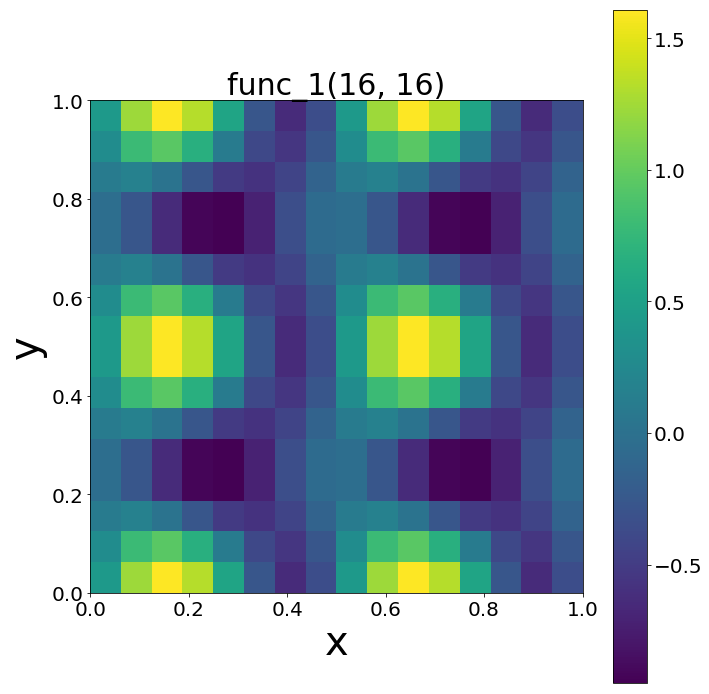
\includegraphics[width=0.7\linewidth]{results/fft_func_1(16,16).png}} 
				\end{minipage}
				\hfill
				\begin{minipage}[h]{0.47\linewidth}
					\center{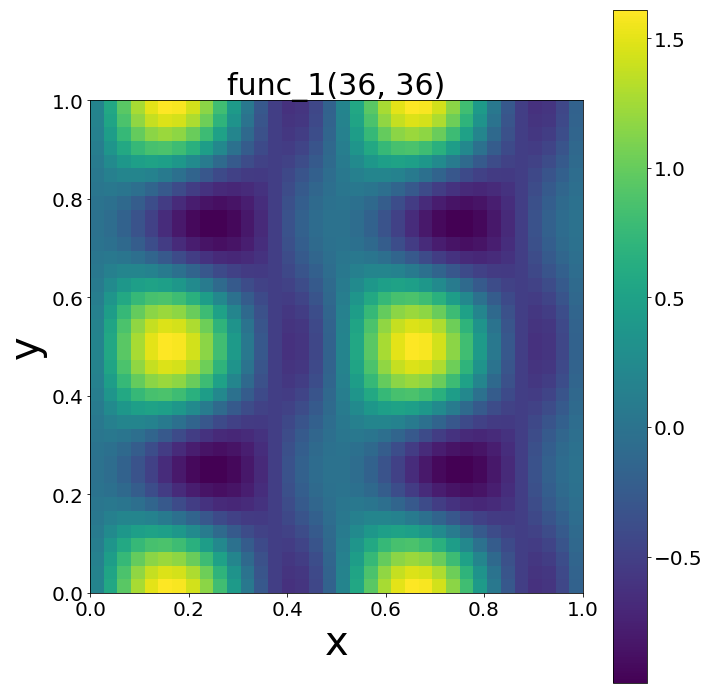
\includegraphics[width=0.7\linewidth]{results/fft_func_1(36,36).png}} 
				\end{minipage}
				\vfill
				\begin{minipage}[h]{0.47\linewidth}
					\center{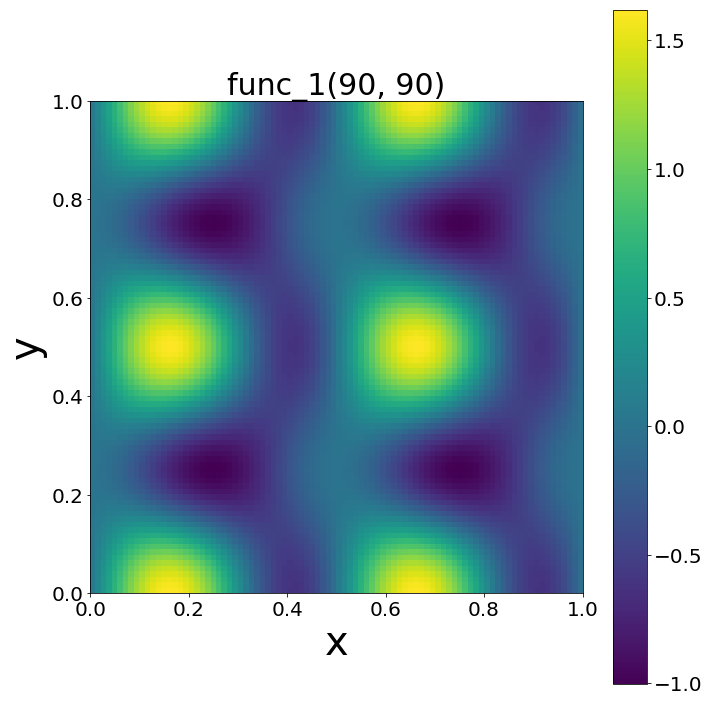
\includegraphics[width=0.7\linewidth]{results/fft_func_1(90,90).png}}
				\end{minipage}
				\hfill
				\begin{minipage}[h]{0.47\linewidth}
					\center{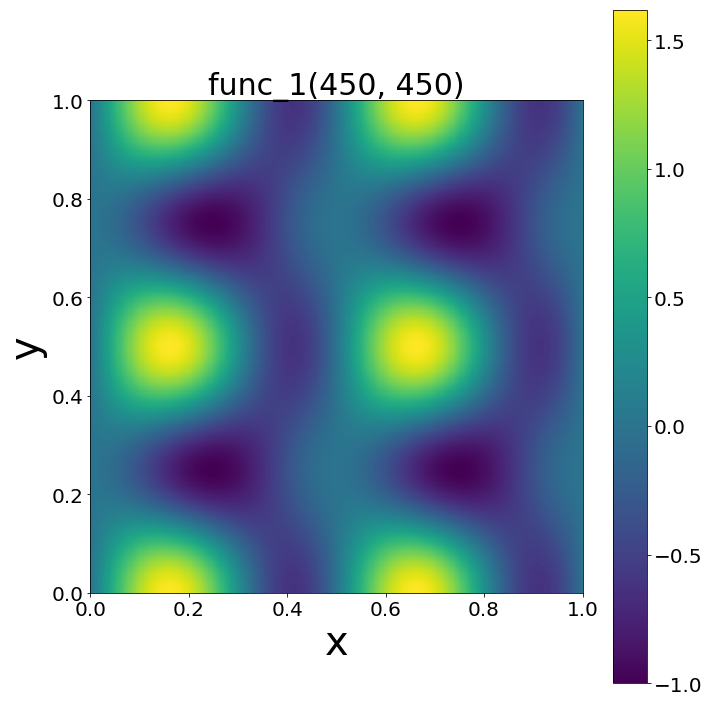
\includegraphics[width=0.7\linewidth]{results/fft_func_1(450,450).png}}
				\end{minipage}
				\caption{График зависимости решения уравнения (1) от числа узлов в создаваемой сетке.}
				\label{ris:func_1_res}
			\end{figure}
		
				\begin{figure}[H]
				\center{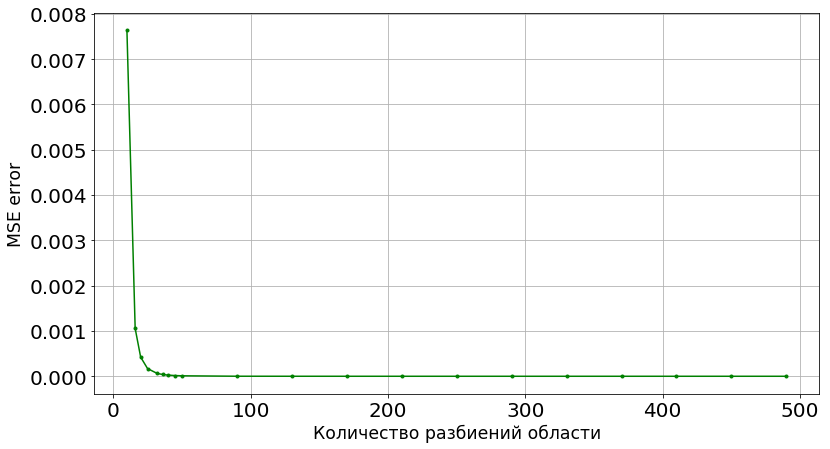
\includegraphics[width=0.8\linewidth]{results/fft_loss_func_1.png}}
				\caption{График зависимости ошибки от количества разбиений области для уравнения (1).}
			\end{figure}
		
		
			\begin{figure}[H]
				\begin{minipage}[h]{0.47\linewidth}
					\center{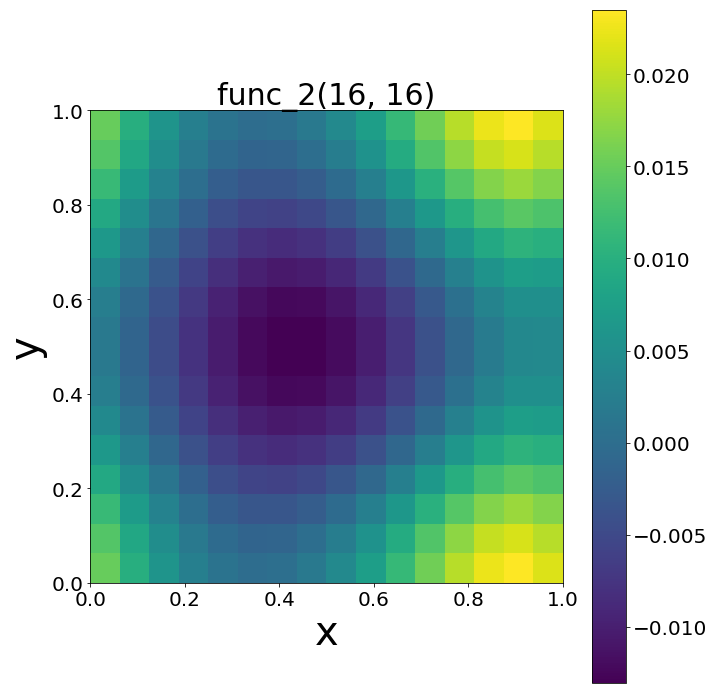
\includegraphics[width=0.7\linewidth]{results/fft_func_2(16,16).png}} 
				\end{minipage}
				\hfill
				\begin{minipage}[h]{0.47\linewidth}
					\center{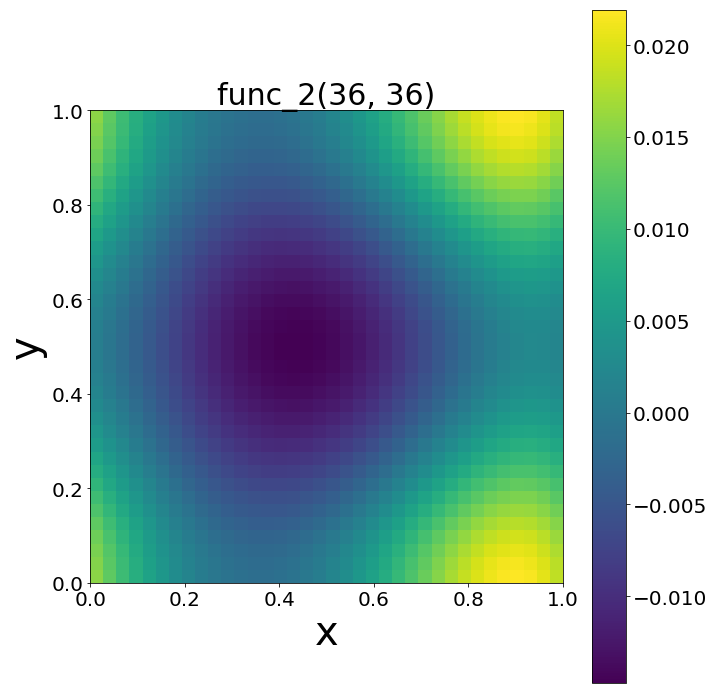
\includegraphics[width=0.7\linewidth]{results/fft_func_2(36,36).png}} 
				\end{minipage}
				\vfill
				\begin{minipage}[h]{0.47\linewidth}
					\center{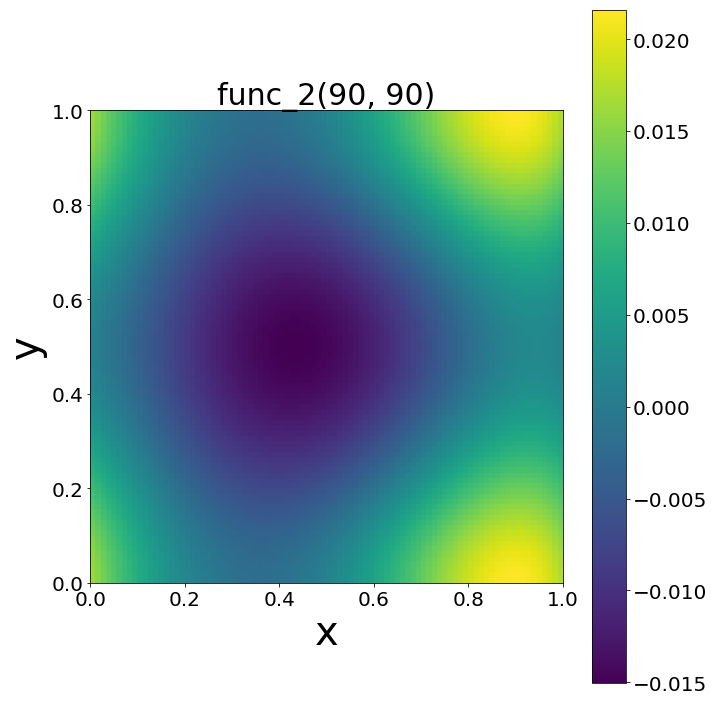
\includegraphics[width=0.7\linewidth]{results/fft_func_2(90,90).png}}
				\end{minipage}
				\hfill
				\begin{minipage}[h]{0.47\linewidth}
					\center{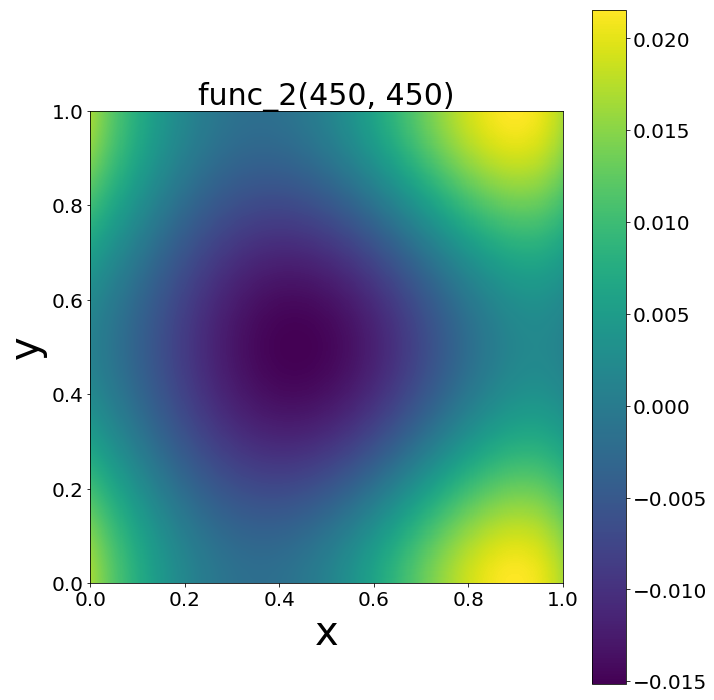
\includegraphics[width=0.7\linewidth]{results/fft_func_2(450,450).png}}
				\end{minipage}
				\caption{График зависимости решения уравнения (2) от числа узлов в создаваемой сетке.}
				\label{ris:func_2_res}
			\end{figure}
		
		\begin{figure}[H]
			\center{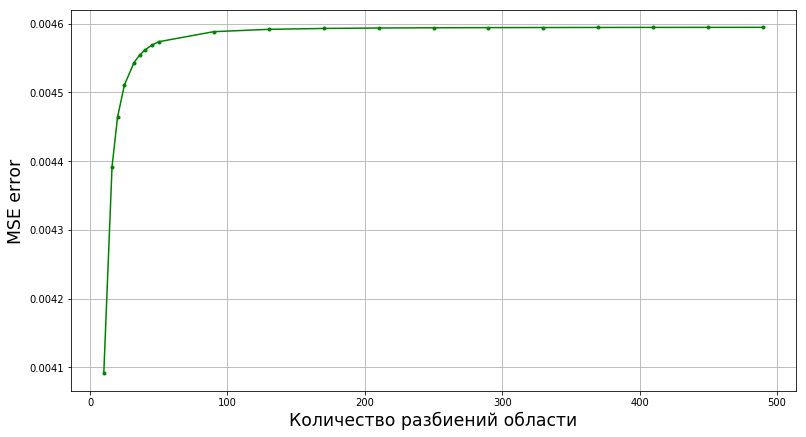
\includegraphics[width=0.8\linewidth]{results/fft_loss_func_2.png}}
			\caption{График зависимости ошибки от количества разбиений области для уравнения (2).}
		\end{figure}
		
		
			\begin{figure}[H]
				\begin{minipage}[h]{0.47\linewidth}
					\center{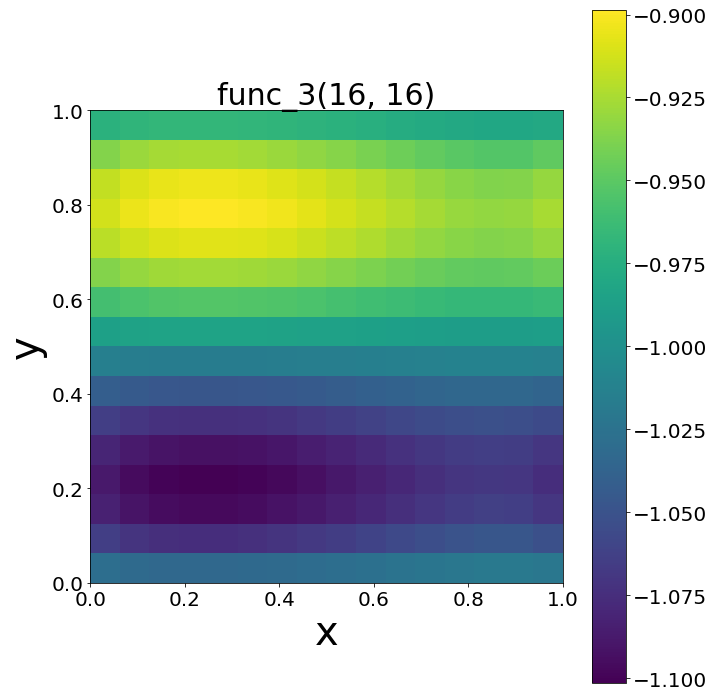
\includegraphics[width=0.7\linewidth]{results/fft_func_3(16,16).png}} 
				\end{minipage}
				\hfill
				\begin{minipage}[h]{0.47\linewidth}
					\center{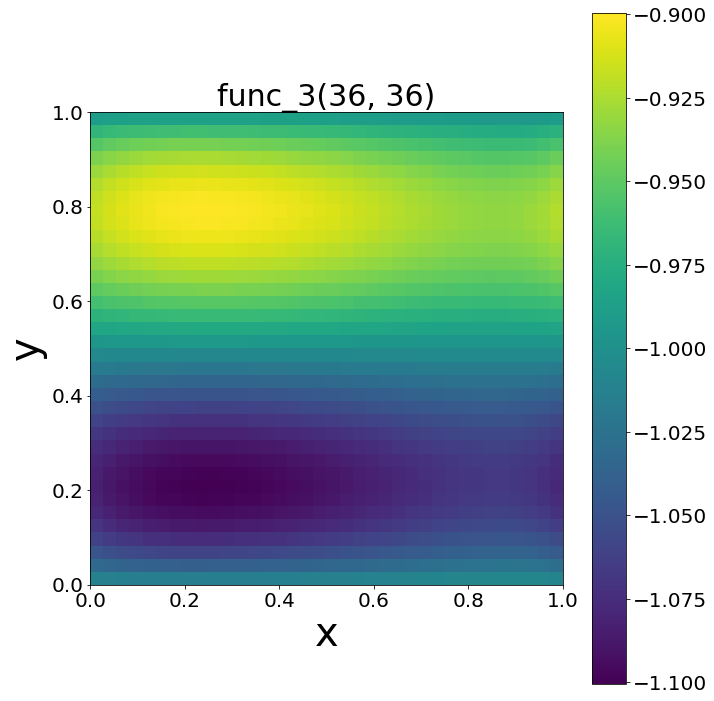
\includegraphics[width=0.7\linewidth]{results/fft_func_3(36,36).png}} 
				\end{minipage}
				\vfill
				\begin{minipage}[h]{0.47\linewidth}
					\center{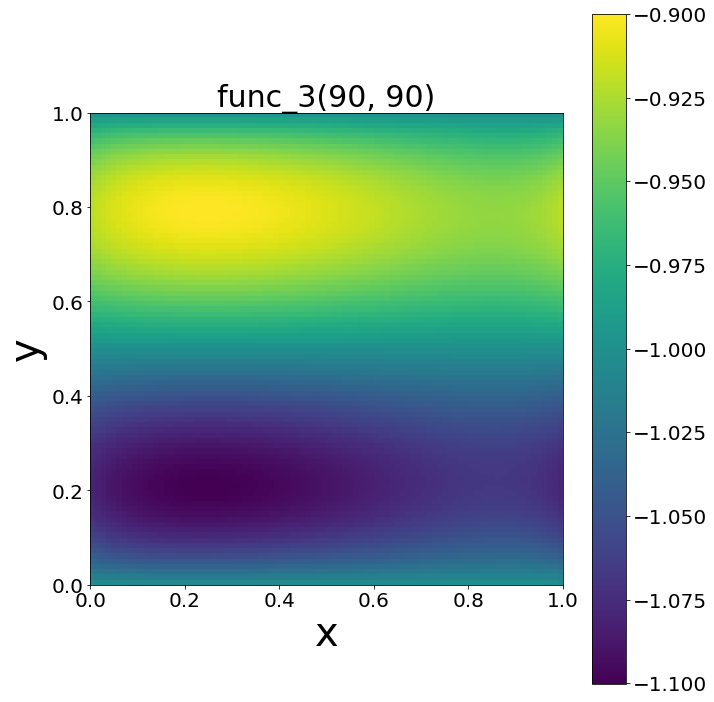
\includegraphics[width=0.7\linewidth]{results/fft_func_3(90,90).png}}
				\end{minipage}
				\hfill
				\begin{minipage}[h]{0.47\linewidth}
					\center{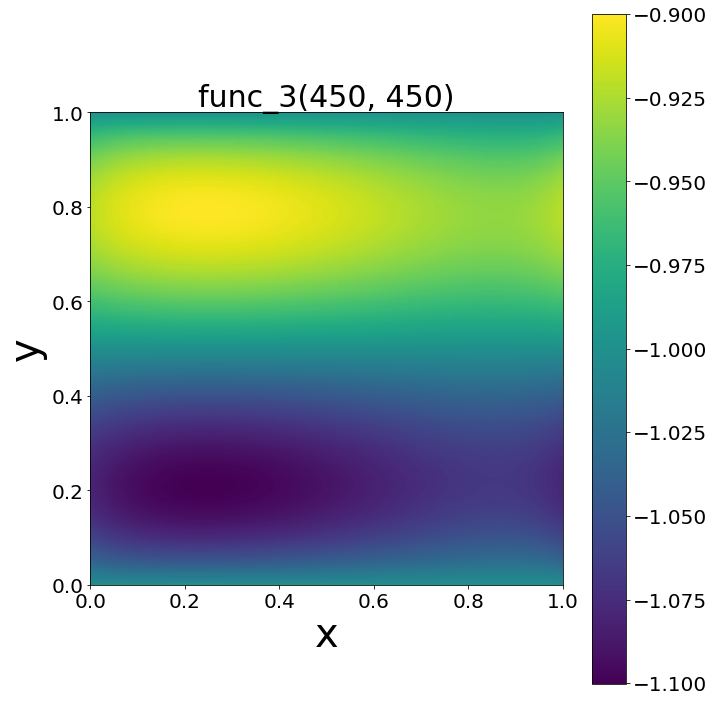
\includegraphics[width=0.7\linewidth]{results/fft_func_3(450,450).png}}
				\end{minipage}
				\caption{График зависимости решения уравнения (3) от числа узлов в создаваемой сетке.}
				\label{ris:func_3_res}
			\end{figure}
		
		\begin{figure}[H]
			\center{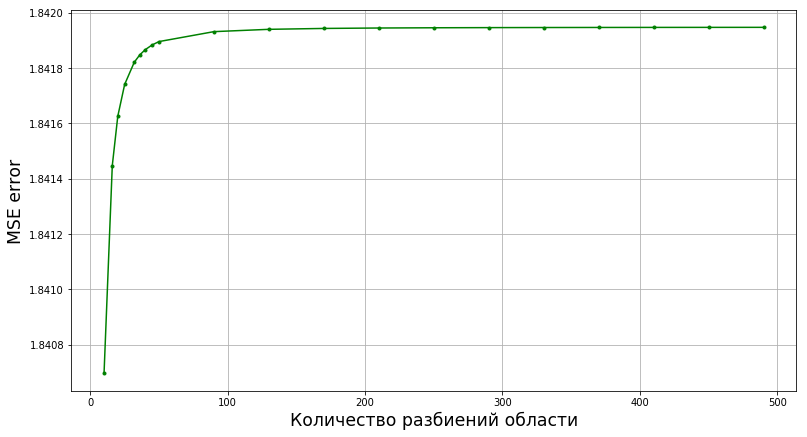
\includegraphics[width=0.8\linewidth]{results/fft_loss_func_3.png}}
			\caption{График зависимости ошибки от количества разбиений области для уравнения (3).}
		\end{figure}
		
		
		\begin{figure}[H]
			\center{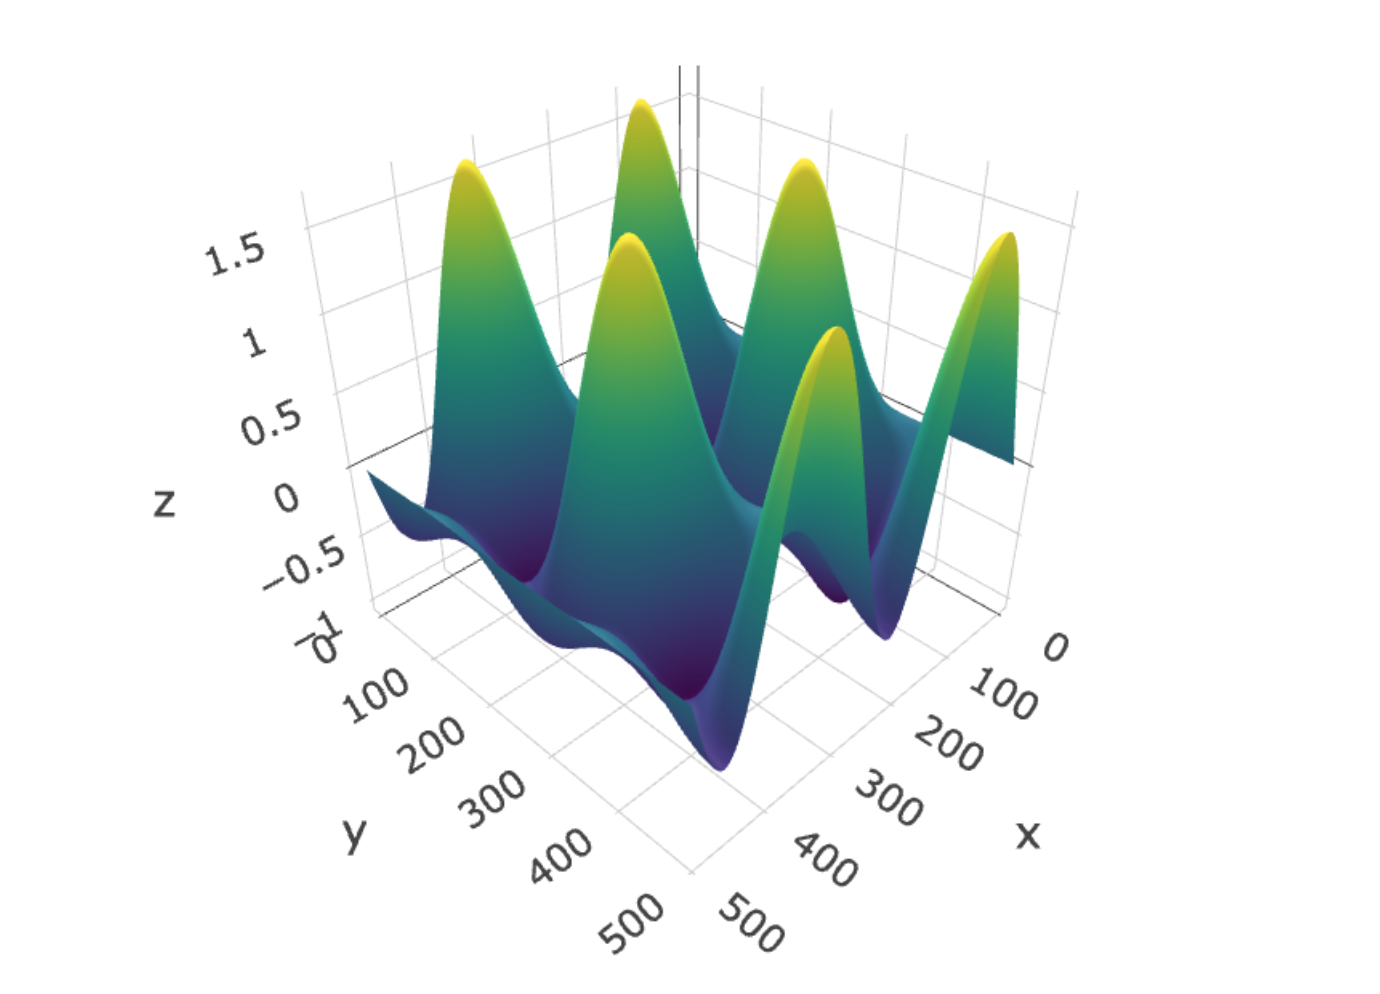
\includegraphics[width=0.85\linewidth]{results/func1_3D.png}}
			\caption{Иллюстрация решения уравнения (1) в $\textit{3D}$.}
		\end{figure}
		 
		 	\begin{figure}[H]
		 	\center{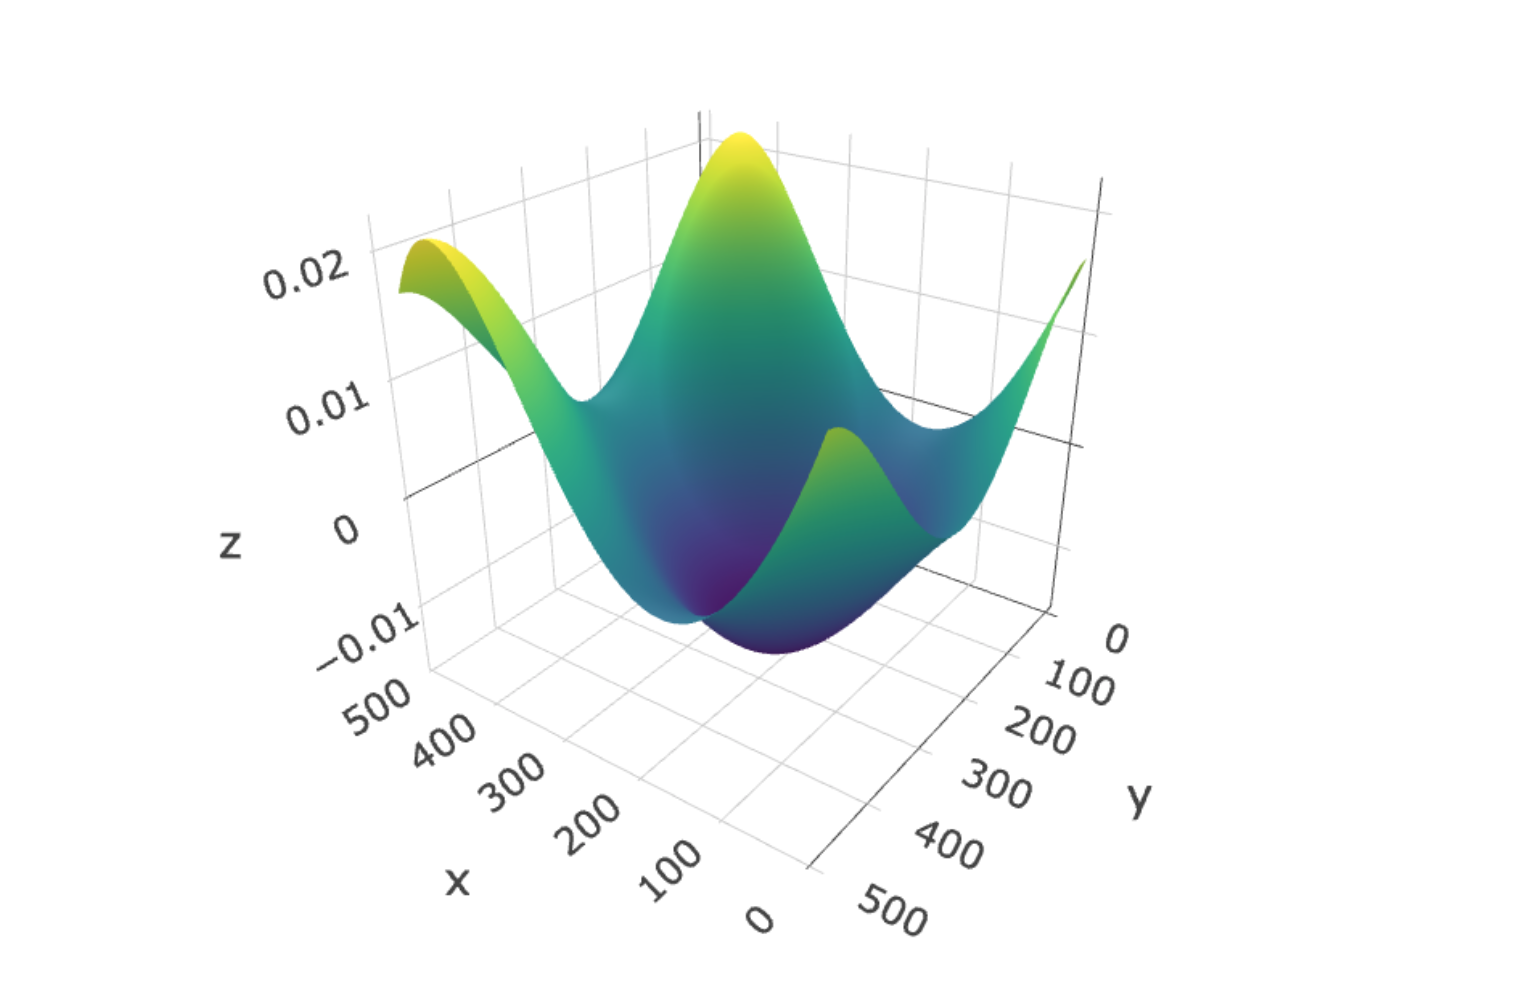
\includegraphics[width=0.85\linewidth]{results/func2_3D.png}}
		 	\caption{Иллюстрация решения уравнения (2) в $\textit{3D}$.}
		 \end{figure}
		 
		 	\begin{figure}[H]
		 	\center{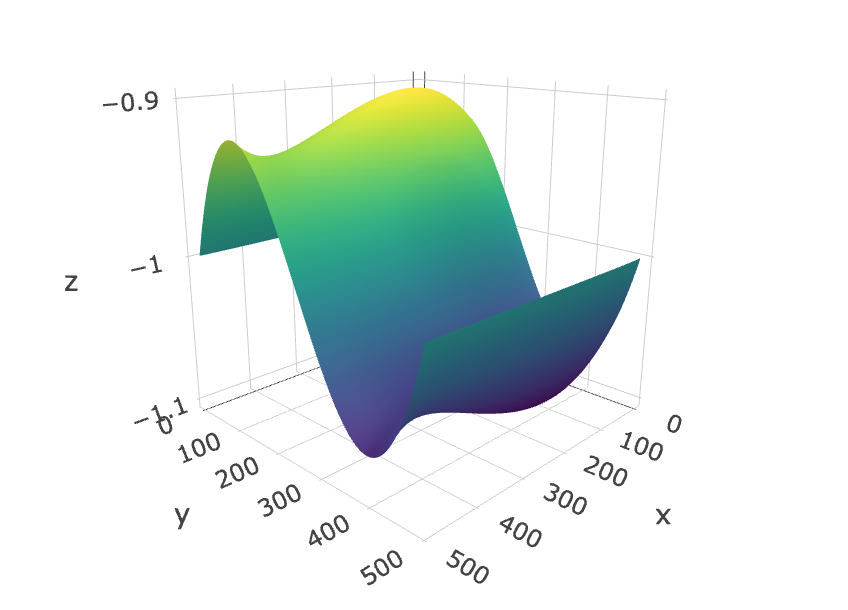
\includegraphics[width=0.85\linewidth]{results/func3_3D.png}}
		 	\caption{Иллюстрация решения уравнения (3) в $\textit{3D}$.}
		 \end{figure}
		 
	\newpage
	\section{Заключение}
	
	В данной работе нами был рассмотрен способ решения двумерного уравнения Пуассона методом быстрого преобразования Фурье. Анализ ошибки говорит о том, что данный метод крайне точно решает поставленную задачу. При увеличении количества разбиений на сетке ошибка мало менялась.  
	
	\begin{thebibliography}{3} 
		\bibitem{cormen} \textit{Thomas Cormen, Charles E.Leiserson, Ronald L.Rivest, Clifford Stein N.} Introduction to Algorithms // MIT, 3rd edition, 2013, Pp.952-962.
		
		\bibitem{nemec} \textit{Kasper Ornstein Mecklenburg N.}Creating Visual Effects by Solving Partial Differential Equations in Real-Time // Bachelor's thesis, 2014
		
		\bibitem{presentation} \textit{Dr. Richard J. Gonsalves N.} Solving Poisson's Equation using the FFT // SUNY Buffalo State College, 2009 
	\end{thebibliography}
	
 
\end{document} 	